\section{はじめに}

この文章は、\cite{grisetti2010}などのチュートリアルを見ても数式の細かいところが分からない
graph-based SLAMについて、
実際の計算方法を細かく解説するためのものです。

\section{問題}

%対向二輪型(その場で回転できるロボット)で、
平面上を移動し、向きを持ち、カメラでランドマーク観測ができるロボットで
graph-based SLAMを実行する方法を考える。ランドマークは環境にいくつか存在し、
ロボットからは互いに識別でき、距離と見える方角が観測できる。
また、2つの観測がどの方角から観測されたものか、相対的に分かるものとする。

\subsection{ロボットの姿勢と座標系}\label{sub:pose}

世界座標系$\Sigma_\text{w}$におけるロボットの姿勢(位置と向き)を
\begin{align}
	\V{x} =
	\begin{bmatrix}
		x \\ y \\ \theta
	\end{bmatrix}
\end{align}
で表す。また、$[x\ y]^T$を原点として、$X$軸が世界座標系で$\theta$の方向を向いているロボット座標系
$\Sigma_\text{r}$を考える。これらの関係を図\ref{fig:coordinate}に示す。

\begin{figure}[htbp]
	\begin{center}
		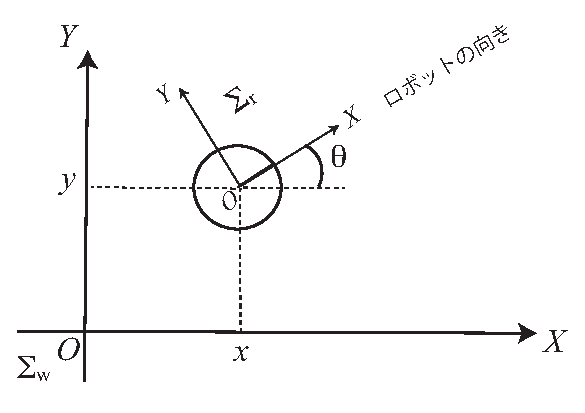
\includegraphics[width=0.5\linewidth]{./figs/coordinate.eps}
		\caption{世界座標系とロボットの姿勢}
		\label{fig:coordinate}
	\end{center}
\end{figure}

%\subsection{ロボットの運動}

離散的な時刻$t = 0,1,2,\dots,T$を考える。
時刻の集合を$\mathcal{T}$で表す。
時刻$t$における世界座標系でのロボットの姿勢を$\V{x}_t$で表す。
ロボットはデッドレコニングで$\V{x}_t$の推定値$\hat{\V{x}}_t$を認識するが、
ロボットの動作は雑音の影響を受けるため、
$\V{x}_t$と$\hat{\V{x}}_t$の間には誤差が発生する。


ロボットは一つの行動ごとに$\hat{\V{x}}_t$を記録していく。
全時刻の推定姿勢を
\begin{align}
\hat{\V{x}}_{0:T} = \{\hat{\V{x}}_0, \hat{\V{x}}_1, \dots, \hat{\V{x}}_T \}
\end{align}
と表すこととする。

\subsection{観測}

環境中にいくつかランドマークが存在していると仮定する。
時刻$t$におけるロボット座標系$\Sigma_\text{r}$を$\Sigma_{\text{r}t}$と表すこととすると、
ロボットには、時刻$t$において、全ランドマークのうちいくつかを計測する。

\subsubsection{ランドマークの識別}

ロボットからは、一度観測したランドマークは、後の時刻で観測したときに、どのランドマークか
識別できることとする。ロボットは観測したランドマークにIDを与えて管理することにする。
IDは$c$と表し(番号でも文字列でもなんでも良い)、IDとして$c$を与えられたランドマークを
$L_c$と表す。
ロボットが認識しているランドマークのIDの集合を$C$で表す。

\subsubsection{ランドマークの位置計測}

ロボットは$\Sigma_{\text{r}t}$においてランドマーク$L_c$を観測したとき、
$L_c$までの距離$d_{c,t}$と、ランドマークが見える方向$\varphi_{c,t}$を計測値として得る。
図\ref{fig:observation}にこれらの記号の関係を示す。

\begin{figure}[htbp]
	\begin{center}
		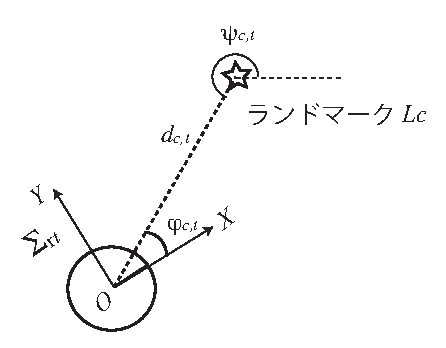
\includegraphics[width=0.5\linewidth]{./figs/observation.eps}
		\caption{計測値}
		\label{fig:observation}
	\end{center}
\end{figure}

また、ランドマークにはなんらかの模様がついていて、2箇所からの計測値から、
ランドマークの面を観測したか相対的に分かると仮定する。
この相対的な向きの差を図\ref{fig:observation}のように$\psi_{c,t,t'}$と表す。
向きは、$\theta, \varphi, \psi$共に反時計回りを正とする。


\subsubsection{計測値の記録}

ロボットが時刻$t$で得るランドマーク全ての計測値の集合は、
$Z_t = \{ \V{z}_{c,t} = (d_{c,t}, \varphi_{c,t}) |
c \in C, c\text{: 観測したランドマークのID} \}$
で表すことができ、これもロボットは各時刻ごとに記録する。
$Z_t$の集合を$Z_{0:T}$で表す。


また、$\psi$の計算のため、センサからの生データ
(ランドマークを写したカメラ画像などの元データ)も保存しておく。
元データからは、ロボットの行動後に、
$\psi$の計測値の集合
$\Psi = \{ \psi_{c,t,t'} | \forall c \in C, \forall t \in \mathcal{T} ,\forall t' \in \mathcal{T},
t \neq t'\}$を作る。


\subsection{完全SLAM問題}

ここで、$Z_{0:T}, \Psi$から、推定値$\hat{\V{x}}_{0:T}$を
真値$\V{x}_{0:T}$に近づける最適化問題を考える。
最適化のための評価関数については後述する。

\section{graph-based SLAMの実装例}

